\documentclass{beamer}
\usepackage[english,russian]{babel}
\usepackage[utf8]{inputenc}
\usepackage{amsmath}
\usepackage{hyperref}
\usetheme{Warsaw}
\usepackage{listings}
\usepackage{xcolor}
\usepackage{tikz}
\usetikzlibrary{graphs}
\usepackage{algpseudocode}

\lstset{
    frame=tb,
    tabsize=4,
    showstringspaces=false,
    numbers=left,
    commentstyle=\color{green},
    keywordstyle=\color{blue},
    stringstyle=\color{red},
    emph={baz},
    emphstyle=\textbf
}

\begin{document}

\title{Задачи разрешимости логических формул и приложения\newline Лекция 7. Логика массивов}
\author{Роман Холин}
\institute{Московский государственный университет}
\date{Москва, 2022}

\begin{frame}
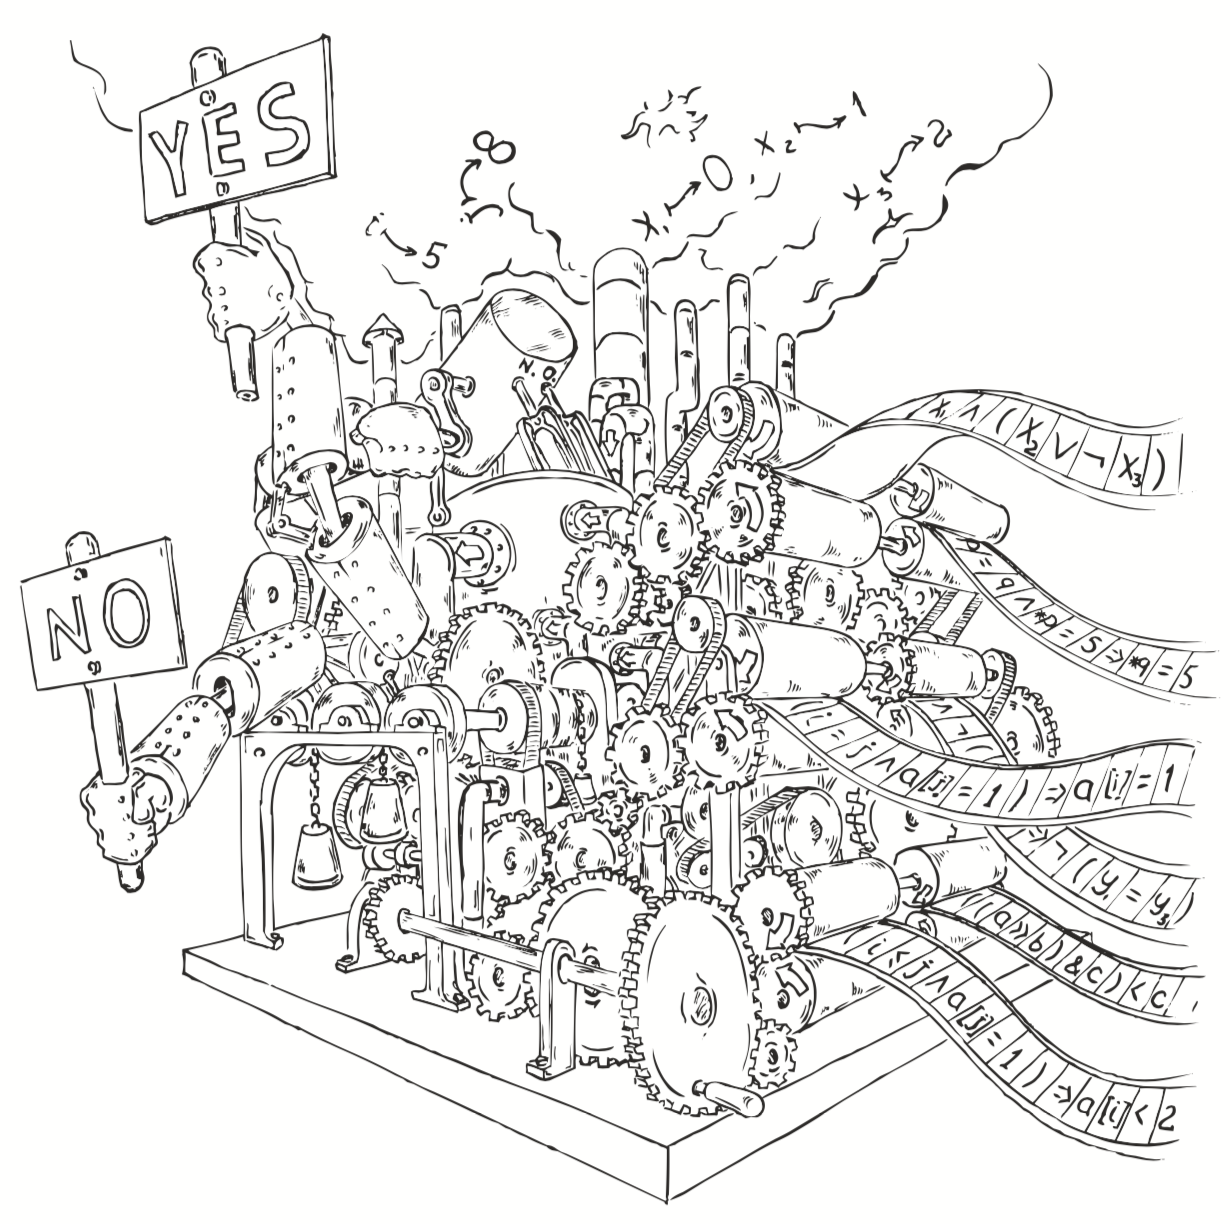
\includegraphics[scale=0.5]{../decision-procedure.png}
\end{frame}

\frame{\titlepage}

\begin{frame}{Пример}
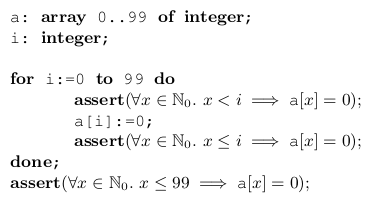
\includegraphics[scale=0.5]{code.png}
\end{frame}

\begin{frame}{Пример}
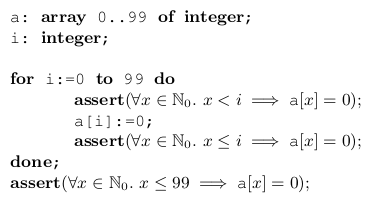
\includegraphics[scale=0.5]{code.png}
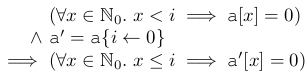
\includegraphics[scale=0.5]{conditions.png}
\end{frame}

\begin{frame}{$a\{i\leftarrow x\}$}
$a\{i\leftarrow x\}$ - присвоить $x$ элементу массива с индексом $i$\newline
\end{frame}

\begin{frame}{$a\{i\leftarrow x\}$}
$a\{i\leftarrow x\}$ - присвоить $x$ элементу массива с индексом $i$\newline
$(\forall x \in \mathbb{N}_0. x < i \implies a[x] = 0) \wedge a' = a\{i\leftarrow 0\} \implies$\newline
$(\forall x \in \mathbb{N}_0. x \le i \implies a'[x] = 0)$
\end{frame}

\begin{frame}{Синтаксис}
$T_I$ - тип индекса\newline
$T_E$ - тип элемента\newline
$T_A$ - тип массива, сокращение от $T_I \rightarrow T_E$ - т.е. множество функций из индексы в элементы\newline
\end{frame}

\begin{frame}{Синтаксис}
$T_I$ - тип индекса\newline
$T_E$ - тип элемента\newline
$T_A$ - тип массива, сокращение от $T_I \rightarrow T_E$ - т.е. множество функций из индексы в элементы\newline
Теория массивов параметризирована теориями индексов и элементов.
\end{frame}

\begin{frame}{Синтаксис}
term A : array-identifier | term$_A\{$term$_I \leftarrow$ term$_E\}$\newline
term E : term$_A[$term$_I]$ | \dots\newline
formula : term$_A$ = term$_A$ | \dots\newline
\end{frame}

\begin{frame}{Семантика}
Аксиома чтения:
$\forall a_1 \in T_A. \forall a_2 \in T_A. \forall i \in T_I. \forall j \in T_I. (a_1 = a_2 \wedge i = j) \implies$\newline
$a_1[i] = a_2[j]$\newline
Аксиома записи:
$\forall a \in T_A. \forall e \in T_E. \forall i \in T_I. \forall j \in T_I. a\{i\leftarrow e\}[j] = (i = j)? e : a[j]$\newline
Аксиома существования:\newline
$\forall a_1 \in T_A. \forall a_2 \in T_A. (\forall i \in T_I. a_1[i] = a_2 [i]) \implies$\newline
$a_1 = a_2$
\end{frame}

\begin{frame}{Пример элиминация термов}
$(i = j \wedge a[j] = 'z') \implies a[i] = 'z'$\newline
\end{frame}

\begin{frame}{Пример элиминация термов}
$(i = j \wedge a[j] = 'z') \implies a[i] = 'z'$\newline
$(i = j \wedge F_a(i) = 'z') \implies F_a(i) = 'z'$\newline
\end{frame}

\begin{frame}{Правило записи}
Перепишем формулу:\newline
для $a\{i\leftarrow e\}$ добавим $a'$, т.ч. $a'[i] = e$ и $\forall j\ne i. a'[j] = a[j]$\newline
\end{frame}

\begin{frame}{Правило записи}
Перепишем формулу:\newline
для $a\{i\leftarrow e\}$ добавим $a'$, т.ч. $a'[i] = e$ и $\forall j\ne i. a'[j] = a[j]$\newline
$a[0] = 10 \implies a\{1 \leftarrow 20\}[0] = 10$\newline
\end{frame}

\begin{frame}{Правило записи}
Перепишем формулу:\newline
для $a\{i\leftarrow e\}$ добавим $a'$, т.ч. $a'[i] = e$ и $\forall j\ne i. a'[j] = a[j]$\newline
$a[0] = 10 \implies a\{1 \leftarrow 20\}[0] = 10$\newline
$(a[0] = 10 \wedge a'[1] = 20 \wedge (\forall j \ne 1. a'[j] = a[j])) \implies a_0[0] = 10$\newline
$(F_a(0) = 10 \wedge F_{a'}(1) = 20 \wedge (\forall j \ne 1. F_{a'}(j) = F_a(j))) \implies F_{a'}(0) = 10$\newline
\end{frame}

\begin{frame}{Правило записи}
Перепишем формулу:\newline
для $a\{i\leftarrow e\}$ добавим $a'$, т.ч. $a'[i] = e$ и $\forall j\ne i. a'[j] = a[j]$\newline
$a[0] = 10 \implies a\{1 \leftarrow 20\}[0] = 10$\newline
$(a[0] = 10 \wedge a'[1] = 20 \wedge (\forall j \ne 1. a'[j] = a[j])) \implies a_0[0] = 10$\newline
\end{frame}

\begin{frame}{Свойство массива}
$\forall i_1 \dots \forall i_k \in T_I. \phi_I(i_1, \dots, i_k) \implies \phi_V(i_1, \dots, i_k)$\newline
\end{frame}

\begin{frame}{Свойство массива}
$\forall i_1 \dots \forall i_k \in T_I. \phi_I(i_1, \dots, i_k) \implies \phi_V(i_1, \dots, i_k)$\newline
1) Грамматика для $\phi_I$:\newline
iguard : iguard $\wedge$ iguard | iguard $\vee$ iguard | iterm $\le$ iterm | iterm $=$ iterm\newline
iterm : $i_1$ | $\dots$ | $i_k$ | term\newline
term : integer-constant | integer-constant $\times$ index-identifier | term $+$ term\newline
index-identifier и term не могут быть $i_1, \dots, i_k$\newline
2) $i_1, \dots, i_k$ могут быть только частью выражения чтения вида $a[i_j]$\newline
\end{frame}

\begin{frame}{Пример}
$a' = a\{i\leftarrow 0\}$\newline
\end{frame}

\begin{frame}{Пример}
$a' = a\{i\leftarrow 0\}$\newline
$\forall j \ne i. a'[j] = a[j]$\newline
\end{frame}

\begin{frame}{Пример}
$a' = a\{i\leftarrow 0\}$\newline
$\forall j \ne i. a'[j] = a[j]$\newline
$\forall j. (j \le i - 1 \wedge i + 1 \le j) \implies a'[j] = a[j]$
\end{frame}

\begin{frame}{$\iota(\phi)$}
$\iota(\phi)$ - множество элементов, которые могут быть равны какому-нибудь индексу, т.е.:\newline
1) Все выражения, которые используются как индекс массива и которые не связаны квантором\newline
2) Все выражения, которые используются внутри ограничений на индексы и которые не связаны квантором\newline
3) Если $\phi$ ничего такого не содержит, то $\iota(\phi) = \{0\}$, чтобы оно не было пусто\newline
\end{frame}

\begin{frame}{Редукция массивов}
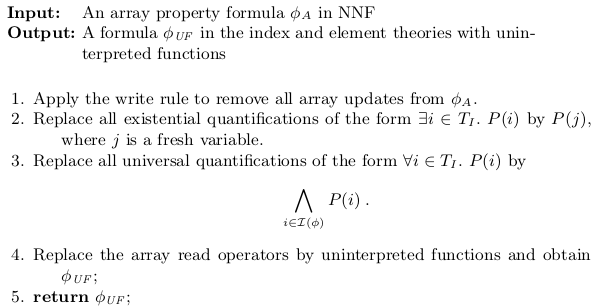
\includegraphics[scale=0.5]{array-reduction.png}
\end{frame}

\begin{frame}{Пример}
$(\forall x \in \mathbb{N}_0. x < i \implies a[x] = 0) \wedge a' = a\{i\leftarrow 0\} \implies$\newline
$(\forall x \in \mathbb{N}_0. x \le i \implies a'[x] = 0)$
\end{frame}

\begin{frame}{Пример}
$(\forall x \in \mathbb{N}_0. x < i \implies a[x] = 0) \wedge a' = a\{i\leftarrow 0\} \implies$\newline
$(\exists x \in \mathbb{N}_0. x \le i \wedge a'[x] \ne 0)$
\end{frame}

\begin{frame}{Пример}
$(\forall x \in \mathbb{N}_0. x < i \implies a[x] = 0) \wedge a'[i] = 0 \wedge \forall j \ne i. a'[j] = a[j] \implies$\newline
$(\exists x \in \mathbb{N}_0. x \le i \wedge a'[x] \ne 0)$
\end{frame}

\begin{frame}{Пример}
$(\forall x \in \mathbb{N}_0. x < i \implies a[x] = 0) \wedge a'[i] = 0 \wedge \forall j \ne i. a'[j] = a[j] \implies$\newline
$(z \le i \wedge a'[z] \ne 0)$
\end{frame}

\begin{frame}{Пример}
$\iota(\phi) = \{i, z\}$
\end{frame}

\begin{frame}{Пример}
$\iota(\phi) = \{i, z\}$\newline
$(i < i \implies a[i] = 0) \wedge (z < i \implies a[z] = 0) \wedge$\newline
$a'[i] = 0 \wedge \forall j \ne i. a'[j] = a[j] \implies$\newline
$(z \le i \wedge a'[z] \ne 0)$
\end{frame}

\begin{frame}{Пример}
$\iota(\phi) = \{i, z\}$\newline
$(i < i \implies a[i] = 0) \wedge (z < i \implies a[z] = 0) \wedge$\newline
$a'[i] = 0 \wedge (i \ne i \implies a'[i] = a[i]) \wedge (z \ne i \implies a'[z] = a[z])\implies$\newline
$(z \le i \wedge a'[z] \ne 0)$
\end{frame}

\begin{frame}{Пример}
$(z < i \implies a[z] = 0) \wedge$\newline
$a'[i] = 0 \wedge (z \ne i \implies a'[z] = a[z])\implies$\newline
$(z \le i \wedge a'[z] \ne 0)$
\end{frame}

\begin{frame}{Пример}
$(z < i \implies F_a(z) = 0) \wedge$\newline
$F_{a'}(i) = 0 \wedge (z \ne i \implies F_{a'}(z) = F_a(z))\implies$\newline
$(z \le i \wedge F_{a'}(z) \ne 0)$
\end{frame}

\begin{frame}{}
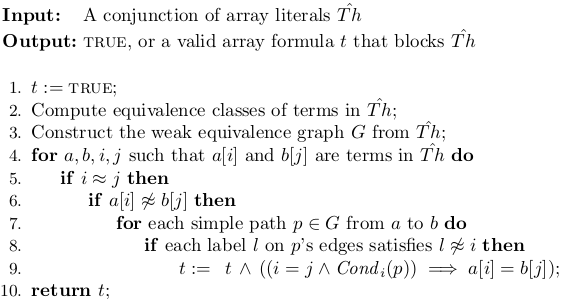
\includegraphics[scale=0.5]{array-encoding-procedure.png}
\end{frame}

\begin{frame}{}
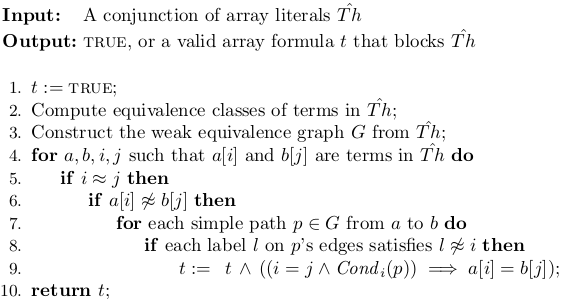
\includegraphics[scale=0.5]{array-encoding-procedure.png}
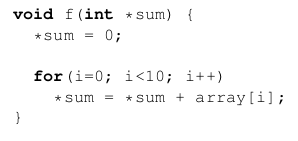
\includegraphics[scale=0.5]{ex1.png}
\end{frame}

\begin{frame}{}
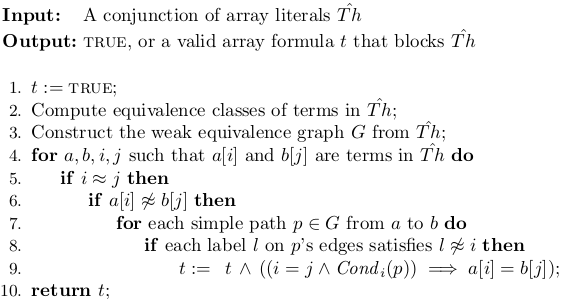
\includegraphics[scale=0.5]{array-encoding-procedure.png}
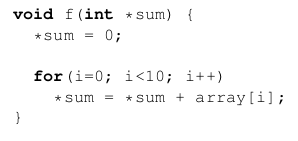
\includegraphics[scale=0.5]{ex1.png}
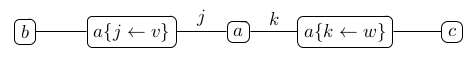
\includegraphics[scale=0.5]{graph1.png}
\end{frame}

\begin{frame}{}
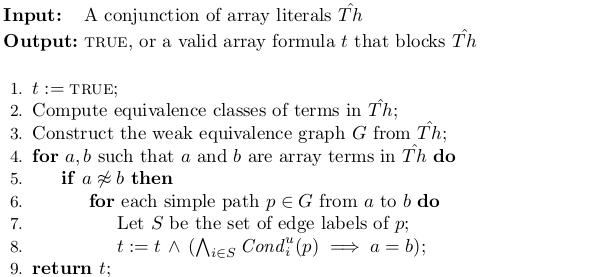
\includegraphics[scale=0.5]{extensional-array-encoding.png}
\end{frame}

\begin{frame}{}
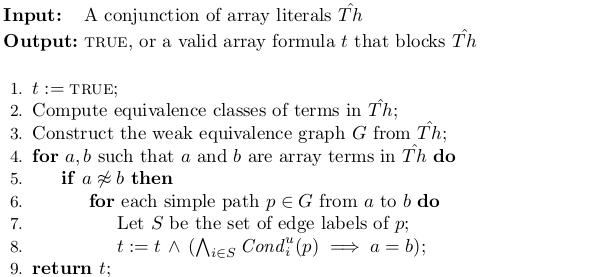
\includegraphics[scale=0.5]{extensional-array-encoding.png}
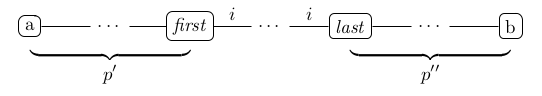
\includegraphics[scale=0.5]{graph2.png}
\end{frame}

\begin{frame}{}
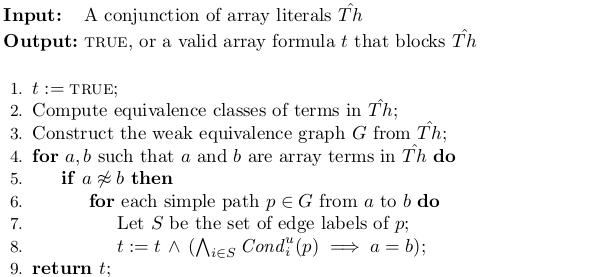
\includegraphics[scale=0.5]{extensional-array-encoding.png}
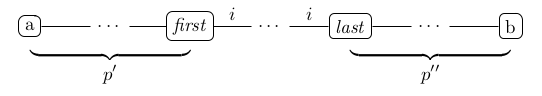
\includegraphics[scale=0.5]{graph2.png}
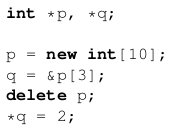
\includegraphics[scale=0.5]{ex2.png}
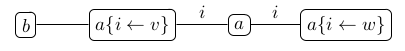
\includegraphics[scale=0.5]{graph3.png}
\end{frame}

\begin{frame}
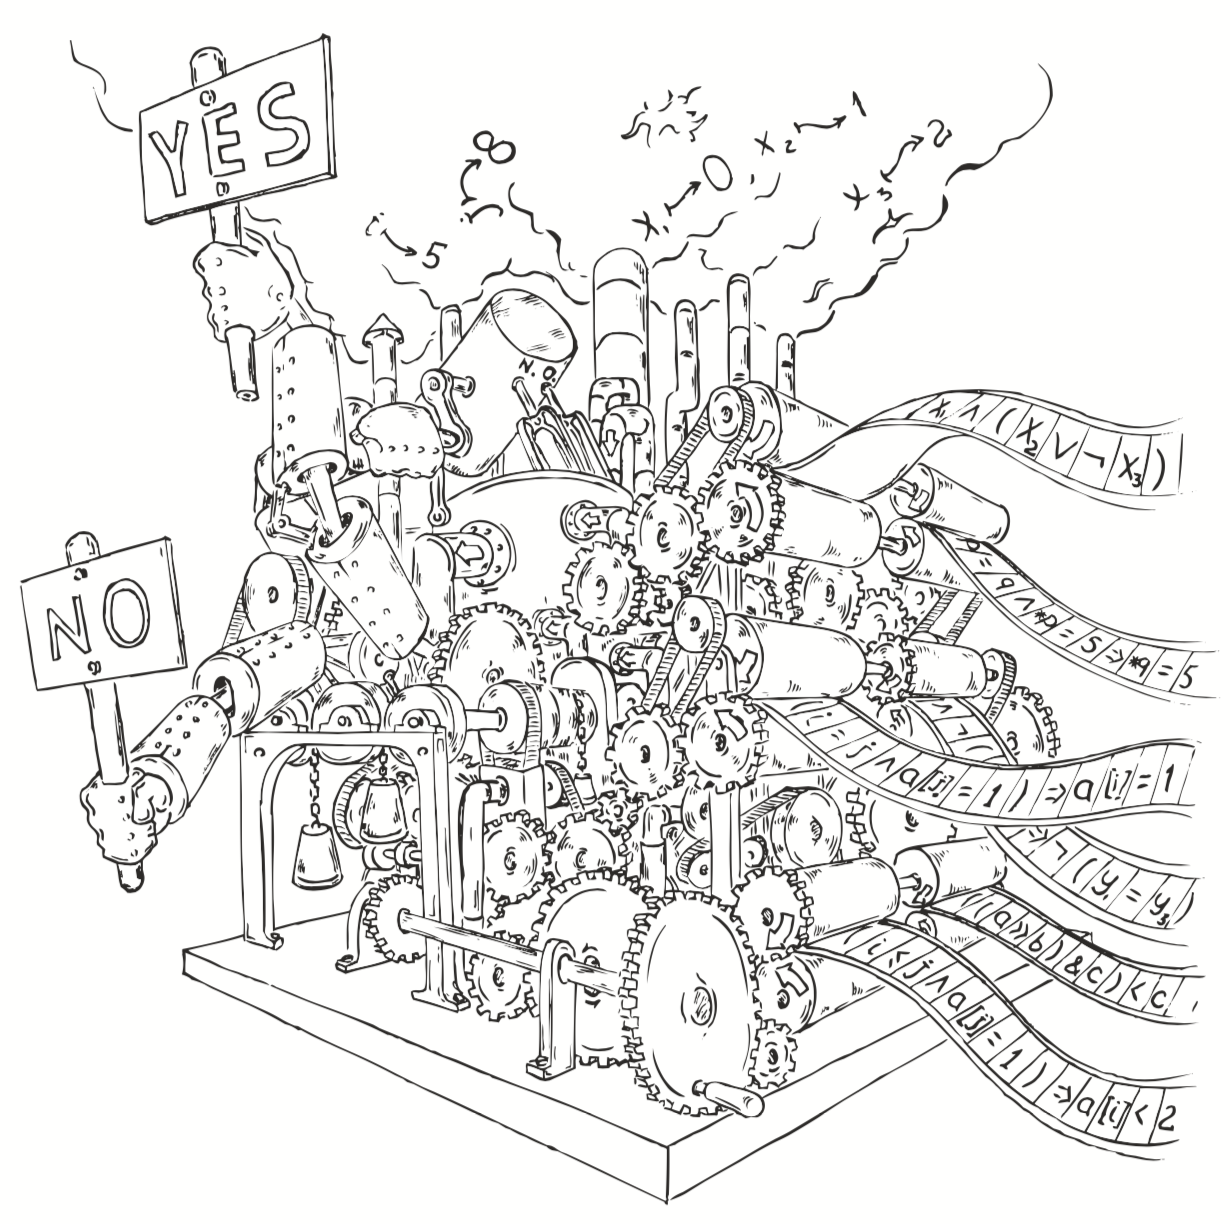
\includegraphics[scale=0.5]{../decision-procedure.png}
\end{frame}

\end{document}
